% declare our document TYPE
\documentclass[12pt]{extarticle}

%%%%%%%% PACKAGES NEEDED FOR THIS DOCUMENT

% allow us to put pictures in the document
\usepackage{graphicx}
% this line lets us use larger fonts
\usepackage{extsizes}
% this allows us to create "slides" in the document
\usepackage[many]{tcolorbox}
% this line lets us caption images inside the "slides"
% this is neccesary since the slide doesn't allow the use of
% \figure{} inside
\usepackage{multicol}
\usepackage{caption}
\usepackage{enumerate}
% allows use of courier font
\usepackage{courier}
% make the table of contents links like people are used to
% the hidelinks parts hides link outlines
\usepackage[hidelinks]{hyperref}
% resize the margins
\usepackage[margin=1in]{geometry}
% use utf8 encoding
\usepackage[utf8]{inputenc}
% one of the other packages complained until I put this here
\usepackage[english]{babel}
% allow citations
\usepackage{cite}
% code listings
\usepackage{listings}
% fix single quote in listings
\usepackage{textcomp}
\usepackage{filecontents}
%\usepackage[noadjust]{cite}
\usepackage{graphicx}
\usepackage{hyperref}
%\hypersetup{
%    colorlinks=true,
%    linkcolor=blue,
%    filecolor=magenta,      
%    urlcolor=cyan,
%}
\usepackage{forest,kantlipsum}
\usepackage{float}
\usepackage{etoolbox}
\usepackage{url}
\usepackage{cleveref}
\usepackage{xcolor}
\usepackage[labelfont=bf]{caption}

%%%%%%%%%%% CUSTOM ENVIRONMENT SETUP

% declare a typesetting environment for code/emphasis
\newcommand{\code}[1]{\texttt{\bfseries#1}}
\newenvironment{codeblock}{\bfseries\texttt\bgroup}{\egroup\par}
% better declaration of font environment
%\DeclareTextFontCommand{\codetext}[1]{\code{#1}}
% declare a large font environment for use in the "slides"
\newcommand{\instruction}[1]{\Large{#1}}
% font environment again
%\DeclareTextFontCommand{\instruction}{\instructionfont}
\newenvironment{instructionblock}{\Large\bgroup}{\egroup}

% declare a "slide" text box for use in the document
% the slide is a numbered \section{}
\newtcolorbox[auto counter]{slide}[3][]{%
colback=brown!5!white,colframe=brown!80!gray,height from=4in to 9in,
title={\addcontentsline{toc}{section}{\thetcbcounter ~~ #2}\bf\Large\thetcbcounter ~ #2\hfill #3 \label{slide \thetcbcounter}\setcounter{section}{\thetcbcounter}}}

% declare a "subslide" text box for use in the document
% the subslide is a numbered \subsection{}
\newtcolorbox[auto counter,number within=section]{subslide}[3][]{%
colback=brown!5!white,colframe=brown!80!gray,height from=4in to 9in,
title={\addcontentsline{toc}{subsection}{\thetcbcounter ~~ #2}\bf\Large\thetcbcounter ~ #2\hfill #3 \label{slide \thetcbcounter}}}

\renewcommand{\labelitemii}{$\circ$}

\lstset{basicstyle=\ttfamily,keywordstyle=\bfseries\color{blue!80!black},identifierstyle=\bfseries,stringstyle=\color{red},showstringspaces=false,commentstyle=\itshape\color{green!40!black},upquote=true}

% My Environments (keep these)
\newcommand{\ben}{\begin{enumerate}}
\newcommand{\een}{\end{enumerate}}
\newcommand{\bi}{\begin{itemize}}
\newcommand{\ei}{\end{itemize}}

%%%%%%%%% SET UP OUR TITLE PAGE

\begin{document}
\title{ Network Firewalls Part II\\ \normalsize Network Firewall Configuration and Management Using pfSense }
\author{Gabe Gibler \& Colton Hotchkiss }
\date{July 15, 2017 \\ \hyperref[changelog]{Version 1.5} }
\renewcommand{\abstractname}{Summary}
\begin{titlepage}
\maketitle
\pagenumbering{gobble}
\begin{center}

\includegraphics[scale=.5]{UofI}

\large{CS 439/CS 539: Applied Security Concepts}

\vskip 40pt

\end{center}
\begin{abstract}
This tutorial focuses on pfSense configuration, weaknesses of default configurations and the mitigation of those weaknesses. Effectiveness of firewalls depends upon how well it is managed and not on how perfectly it is deployed. Therefore, in this tutorial, we will demonstrate management (usage and configuration) of the pfSense firewall.
\end{abstract}


\vfill
\begin{center}
	
\includegraphics[scale=0.5]{cc}
	\vskip 10pt
	This work is licensed under a \href{https://creativecommons.org/licenses/by/4.0/}{Creative Commons Attribution 4.0 International License}.
\end{center}

\end{titlepage}

%%%%%%%%%% TABLE OF CONTENTS

\pagebreak
\tableofcontents

%%%%%%%%%%%%%%%%%%%%%%%%%%%%%%%%%%%%%%%%%%%%%%%%%
%%%%%%    BEGINNING OF MAIN BODY OF DOCUMENT
%%%%%%%%%%%%%%%%%%%%%%%%%%%%%%%%%%%%%%%%%%%%%%%%%

\pagebreak
\pagenumbering{arabic}
\setcounter{section}{1}

%----------------------------------------------------------------------------------------------------%





\begin{slide}{ Objectives of this Tutorial }{ \hyperref[slide 2]{\textgreater} }
	\begin{instructionblock}
		\ben
			\item Review basic pfSense configuration:
			\begin{itemize}
			\item Setup a firewall to manage a LAN, WAN;
			\item Establish ingress and egress filtering rules.
			\end{itemize}
			
			\item Experiment with rules management and network monitoring:
			\begin{itemize}
			\item Configure a restricted firewall and test its configuration;
			\item Find issues with traffic originating from inside the network.
			\end{itemize}
		\een
	\end{instructionblock}
\end{slide}


\vspace{8mm}
\noindent
This tutorial is not a complete user's guide to pfSense management. For that you will want to consult the pfSense wiki. We will briefly explain, through walkthroughs, activities, and challenges, the above objectives.


%----------------------------------------------------------------------------------------------------%





\pagebreak	
\begin{slide}{ Required Background }{ \hyperref[slide 1]{\textless}\hyperref[slide 3]{\textgreater} }
	\begin{instructionblock}
		We assume some knowledge in the following areas:
		\begin{enumerate}
			\item Experience using computers and software applications, like web browsers, and virtualization apps;
			\item Fundamentals of Internet and networking mechanisms like TCP/IP stack, TCP/UDP protocols and ports, etc.;
			\item An introductory knowledge of data privacy, computer/network security, etc.;
			\item Basic wireshark knowledge.
		\end{enumerate}
	\end{instructionblock}
\end{slide}


\vspace{8mm}
\noindent
It is not the goal of this tutorial to be completely self-contained and self-explanatory. As such, the tutorial assumes certain background skills and knowledge. The following are some areas where we expect the users of this tutorial to have some previous skills/knowledge:

\ben

\item Practical experience using computers, and installing and using common software applications (particularly web browsers, and virtualization platforms). The tutorial does not always explain how to navigate within the operating system's graphical user interface (GUI) or how to execute commands from the command line. Some exposure to logic notations and elementary programming skills would be very helpful with writing firewall rules. Similarly, the tutorial does not explain how to browse the Internet, or how to install software applications.

\item Fundamental knowledge of networking mechanisms and computer networks. This tutorial expects a user to understand technical concepts like the ISO OSI model of networks, and common networking terms such as ``packets", ``ports", "protocols", ``accept/drop" in relation to packets, ``TCP" and ``UDP", etc.

\item A broad understanding of general computer-related issues will help, such as ``data privacy", ``network access privileges", ``application permissions", and different sorts of internet-based attacks.

\item Wireshark is software for monitoring, logging and filtering network traffic. It will be used for monitoring and examining network traffic in detail between the VMs. For an introduction to Wireshark, see the other Applied Security Concepts tutorials from the University of Idaho.

\een 


%----------------------------------------------------------------------------------------------------%





\pagebreak
\begin{slide}{ Hardware and Software Requirements }{ \hyperref[slide 2]{\textless}\hyperref[slide 4]{\textgreater} }
    \begin{instructionblock}
    	The tutorial was executed using the following environment:
    	\begin{enumerate}
    		\item A computer capable of hosting at least 3 virtual machines (VMs);
    		\item A virtualization software platform, e.g. VMWare or VirtualBox;
    		\item A) Two pfSense VMs, B) two Ubuntu VMs, C) one Kali linux VM, and D) one VyOS VM(\textsuperscript{D}).
    	\end{enumerate}
    \end{instructionblock}
\end{slide}

\vspace{8mm}
\noindent
The activities and challenges of this tutorial occur in multiple VMs. As such, it is imperative that the user of this tutorial has a machine powerful enough to boot at least 3 virtual machines smoothly at a time, since the pfSense and VyOS machines are not resource intensive. For the sake of consistency, specifics for each VM are given below:

\vspace{4mm}
\noindent
\label{pfSenseSetup}
\textbf{A}) We are using pfSense 2.3.3 64-bit. You can download the latest version \href{https://www.pfsense.org/download/}{\underline{here}}. The instructions to create this VM can be found \href{https://obviate.io/2015/08/31/tutorial-using-vmware-esxi-and-pfsense-as-a-network-firewallrouter/}{\underline{here}}. We installed two packages \textbf{Snort} and \textbf{SquidGuard}, which can be added from within pfSense in the package manager.

\vspace{4mm}
\noindent
\label{UbuntuSetup}
\textbf{B}) We are using Ubuntu 16.04 64-bit. You can download the Ubuntu 16.04 ISO \href{https://www.ubuntu.com/download/desktop}{\underline{here}}. The instructions on how to create the VM in VMware can be found \href{https://kb.vmware.com/selfservice/microsites/search.do?language=en_US&cmd=displayKC&externalId=1002}{\underline{here}}, or for Virtualbox \href{http://www.hacking-tutorial.com/hacking-tutorial/10-steps-how-to-create-kali-linux-virtual-machine-in-virtual-box/}{\underline{here}}. Netcat and Wireshark were installed on both machines.

\vspace{4mm}
\noindent
\label{KaliSetup}
\textbf{C}) We are using Kali Linux version 2016.2 64-bit. You can download the Kali 2016.2 ISO \href{https://www.kali.org/downloads/}{\underline{here}}. The instructions on how to create the VM in VMware can be found \href{http://www.sysadminshowto.com/how-to-install-kali-linux-2-sana-in-vmware-workstation-11-step-by-step-guide/}{\underline{here}}, or for Virtualbox \href{https://docs.oracle.com/cd/E26217_01/E26796/html/qs-create-vm.html}{\underline{here}}.

\vspace{4mm}
\noindent
\label{VyOSSetup}
\textbf{D}) We are using VyOS 1.1.7 64-bit. You can download it \href{http://packages.vyos.net/iso/release/1.1.7/}{\underline{here}} in the form of an ISO or an OVA template that can be directly imported into VMware. For VMware installations using OVA see the \href{https://wiki.vyos.net/wiki/VMWare}{\underline{VyOS wiki}}, and for Virtualbox see \href{https://nbctcp.wordpress.com/2015/01/20/vyatta-os-under-virtualbox-in-gns3/}{\underline{this}}.\\


In addition, a set of scripts are necessary to implement a communication function and its corresponding data leak for the challenges. We utilized netcat to make the connections, and cron jobs to schedule the tasks. 

The first script, on Control, sends a small set of "status" signals along with timestamps from Control to Workstation. It sends the signals every 5 seconds. The script also intermittently sends, about every minute, a randomly generated string of the same length but different content from the status signals. 

The second script, on Workstation, waits for the connection from Control. It saves the status signals to a log file, \textit{/home/seed/Documents/System\_Status.log}, and the leaked data to another hidden file.

A third script, on Workstation, periodically transmits the contents of the hidden file to the Kali workstation in VLAN (Virtual Local Area Network) 0. It used any arbitrary port above 1000.

The final script is the script on the Kali workstation that awaits the outgoing connection from Workstation, and saves the received data to a file in Documents that can be monitored to see if communications are successfully exiting the company LAN.


%----------------------------------------------------------------------------------------------------%





\pagebreak
\begin{slide}{ Network Layout }{ \hyperref[slide 3]{\textless}\hyperref[slide 5]{\textgreater} }
\vskip 5pt
	\begin{instructionblock}
		\begin{center}
			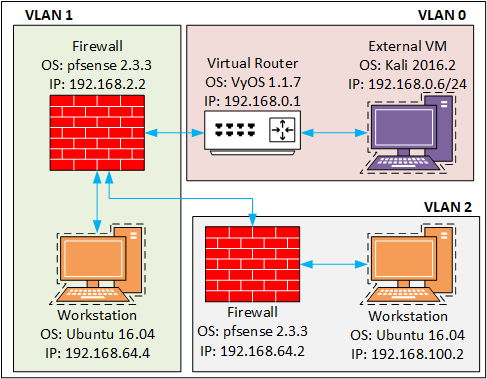
\includegraphics{NetworkDiagram.png}
		\end{center}

	\end{instructionblock}
\end{slide}


%----------------------------------------------------------------------------------------------------%





\pagebreak
\begin{slide}{Firewalls Overview }{ \hyperref[slide 4]{\textless}\hyperref[slide 6]{\textgreater} }
\vskip 5pt
\begin{instructionblock}
\begin{enumerate}
\item What is it?
\begin{enumerate}
\item Hardware and/or software based entity used to protect networks from unauthorized access.
\end{enumerate}
\item What are the main features?
\begin{enumerate}
\item Stateful Packet Inspection;
\item Application Layer Awareness;
\item Network Address Translation (NAT);
\item Virtual Private Networking (VPN).
\end{enumerate}
\end{enumerate}

\end{instructionblock}
\end{slide}


\vspace{8mm}
\ben

\item \textbf{What are they?}
\begin{enumerate}
\item Network firewalls are usually located at the boundary between the internal network and external networks (Perimeter Firewall) or between internal segments of networks (Interior Firewall).
\end{enumerate}
\item \textbf{What are their features?}
\begin{enumerate}
\item Operating in the network layer the firewall examines a packet's header and footer and determines if the packet belongs to a valid session. Using this information the firewall decides if a packet should be forwarded to the internal network or rejected.\cite{Zen2017PacketInsp}
\item Firewalls that are application aware are able to inspect the contents of packets and make decisions based on their knowledge of the pertinent protocols and programs.
\item Network Firewalls are able to change the network address of devices on either side of the firewall to hide the true addresses of devices. This can prevent devices on the outside of a network from being able to probe the true addresses of devices on a network.\cite{UnivHOU2016Firewalls}
\item Network firewalls are able to create encrypted connections using VPNs between themselves. If a host on a network needs to communicate with a host on another network the firewall can establish a secure communication channel with the other host through its firewall.
\end{enumerate}

\een


%----------------------------------------------------------------------------------------------------%





\pagebreak
\begin{slide}{ Defense-in-depth: pfSense packages }{ \hyperref[slide 5]{\textless}\hyperref[slide 7]{\textgreater} }
\vskip 5pt
\begin{instructionblock}
A firewall by itself is not enough. There are over 40 packages available for pfSense to enhance its functionality, including:
\begin{enumerate}
\item Squid - Caching Proxy;
\item SquidGuard - URL Filter;
\item Darkstat - Network Traffic Monitor;
\item Snort - Intrusion Detection;
\item Country Block .
\end{enumerate}
We will use Snort later in this tutorial.
\end{instructionblock}
\end{slide}

\ben
   \item Squid is a caching proxy for the Web that supports HTTP, HTTPS, FTP and others.\cite{Squid2017Squid-cache}
   \item SquidGuard is a URL redirector based on blacklists.
   \item Snort is a rules-based intrusion detection system. It can be used in strictly monitoring mode, in logging mode, or in full intrusion detection mode, to analyze and regulate network traffic. It can do deep-packet inspection, meaning it can analyze the contents of network packets and act upon them using its rules and application awareness.
\een


%----------------------------------------------------------------------------------------------------%





\pagebreak
\begin{slide}{ Activity: Log in to pfSense GUI }{ \hyperref[slide 6]{\textless}\hyperref[slide 8]{\textgreater} }
\vskip 5pt
\begin{instructionblock}
From the Ubuntu Workstation VM:
\begin{enumerate}
    \item Open up a web browser;
    \item Navigate to the pfSense interface, \textbf{192.168.64.1};
    \item Log in:\\
    User: \textbf{admin};\\
    Password: \textbf{pfsense};
    \item What's the first thing that should've happened when setting up a firewall!?
\end{enumerate}
\end{instructionblock}
\end{slide}


\vspace{8mm}
\begin{enumerate}[2]
\item Open a browser and navigate to the webConfigurator for pfSense. Its address is the address of the LAN interface.

If necessary open a console directly for the external pfSense, and find the address listed for the LAN interface.
\item \texttt{admin}/\texttt{pfsense} is the default password for pfSense routers. 

Is it a good idea to change the default password of the built-in admin?

Yes! It is. Change the default password to something of your choosing and record it somewhere safe for the remainder of the tutorial.
\end{enumerate}



%----------------------------------------------------------------------------------------------------%





\pagebreak
\begin{slide}{ Activity: pfSense Setup }{ \hyperref[slide 7]{\textless}\hyperref[slide 9]{\textgreater} }
\vskip 5pt
\begin{instructionblock}
Review configuration of pfSense for our "business" -- this specific domain.

\begin{enumerate}[1]
\item Review the configuration of its interfaces:
\begin{enumerate}
    \item WAN;
    \item LAN.
\end{enumerate}
These are its physical connections to each network segment.

\end{enumerate}
\end{instructionblock}
\end{slide}


\vspace{8mm}
\begin{enumerate}
\item If you got here, then this is probably not news to you. But it's good to know where to check in on this information if something isn't working.
\end{enumerate}



%----------------------------------------------------------------------------------------------------%





\pagebreak
\begin{slide}{ Activity: Firewall Rules }{ \hyperref[slide 8]{\textless}\hyperref[slide 10]{\textgreater} }
\vskip 5pt
\begin{instructionblock}
Review configuration of pfSense for our "business".

\begin{enumerate}[2]
\item Review the current set of rules for each interface:
\begin{enumerate}
    \item WAN (ingress) Firewall Rules;
    \item LAN (egress) Firewall Rules.
\end{enumerate}
These rules apply to either traffic coming into the network (ingress) or leaving the network (egress).

\end{enumerate}
\end{instructionblock}
\end{slide}


\vspace{8mm}
\noindent
What services will need to be allowed for each interface to be able to do its intended function? What are the common functions of the people using this network? Should everything from the inside be allowed out? Are there downsides to blocking all by default?



%----------------------------------------------------------------------------------------------------%





\pagebreak
\begin{slide}{ Challenge 1: Configure a 2nd Internal pfSense }{ \hyperref[slide 9]{\textless}\hyperref[slide 11]{\textgreater} }
\vskip 5pt
\begin{instructionblock}
    You are tasked with setup of a new internal router/firewall for a new fabrication control unit. ``pfSense internal" will be used for this, and must be configured from scratch. The control unit has a monitoring protocol that sends on TCP port 5009. The firewall must only allow traffic in or out on this port.\\

	\textbf{\Large{Deliverables:}}
	\ben
		\item A fully configured instance of pfSense monitoring the connection between the new internal LAN segment and the existing LAN segment;
		\item Its WAN must point to the existing internal network. Assign it 192.168.64.2/24;
		\item Its LAN must point to a new internal network, for which it will be the gateway. Assign it 192.168.100.1/24;
		\item Firewall rules configured to block all traffic except the monitoring transmissions on port 5009 (and the web management ports for pfSense, as well).
	\een

  \vspace{20mm}
  \begin{center}
  \textbf{\Large{Duration: 45 min.} }
  \end{center}

\end{instructionblock}
\end{slide}


\vspace{8mm}
\noindent
\textbf{HINTS:}
\begin{enumerate}
    \item Configuration will begin with a direct console connection to the internal pfSense (not the web interface).
    \item The format of the IP addresses indicates both the IP address of the interface and its network mask (the number of bits in the mask). For example, for 192.168.64.2/24, 192.168.64.2 is the IP address that needs to be assigned to the interface, 24 is the number of bits in the network mask for that network.
    \item If the WAN points to the existing business network, which device must be its gateway -- the gateway for the WAN?
    \item How about the gateway for the LAN? Why don't you set up a gateway for the LAN interface?
    \item This fabrication control unit is very sensitive, so you want to be very restrictive on the range of ports allowed for communication in or out. How do you restrict both incoming and outgoing ports in firewall rules?
    \item Don't forget to specify to each interface to drop all other packets by default.
    \item If it is not already so, don't forget to point the machines that will be operating on this new network to their gateway/router.
\end{enumerate}



%----------------------------------------------------------------------------------------------------%





\pagebreak
\begin{slide}{ Challenge 1 (cont.): Verify the Setup }{ \hyperref[slide 10]{\textless}\hyperref[slide 12]{\textgreater} }
\vskip 5pt
\begin{instructionblock}
  Verify that the firewall is properly configured by checking that you are receiving status updates in the file \textbf{System\_Status.log}, located in \texttt{/home/seed/Documents} on Workstation (not Control).\\
   
  Please, be careful. The system is finicky. Do not edit or save the file! It messes up the running process.
  

	\textbf{\Large{Deliverables:}}
	\ben
		\item The file \textbf{System\_Status.log} should be receiving status updates, and a few select control sequences;
		\item No other communications should succeed through the firewall.
	\een

  \vspace{20mm}
  \begin{center}
  \textbf{\Large{Duration: 10 min.} }
  \end{center}

\end{instructionblock}
\end{slide}


\vspace{8mm}
\noindent
\textbf{HINTS:}
\begin{enumerate}
    \item If the process stops updating, you may need to restart the Workstation and/or Control machines.
\end{enumerate}



%----------------------------------------------------------------------------------------------------%





\pagebreak
\begin{slide}{ Challenge 2: Who's Leaking Sensitive Data? }{ \hyperref[slide 11]{\textless}\hyperref[slide 13]{\textgreater} }
\vskip 5pt
\begin{instructionblock}
    After the new network for the fabrication unit has been running awhile, it becomes apparent to the company that sensitive data is being leaked to competitors. The information has to be coming from the fabrication control unit somehow.\\
    
    Determine, for your part, whether the data leak is happening through your network systems. If it is, what are its sources and destinations?


	\textbf{\Large{Deliverables:}}
	\ben
		\item Observation of unusual control packets and the route they are taking through your network.
	\een

  \vspace{20mm}
  \begin{center}
  \textbf{\Large{Duration: 10-15 min.} }
  \end{center}

\end{instructionblock}
\end{slide}


\vspace{8mm}
\noindent
\textbf{HINTS:}
\begin{enumerate}
	\item What software is very helpful for monitoring traffic on a network?
	\item You can look at the \href{https://wiki.wireshark.org/CaptureFilters}{Wireshark Wiki} for a list of helpful commands.
	\item BTW: if you manage to locate actual files performing this data leak (if said files exist), for the sake of this tutorial, you're not allowed to interfere directly with them (should such files exist, which they don't). (So, P.S., don't go looking!)
\end{enumerate}


%----------------------------------------------------------------------------------------------------%





\pagebreak
\begin{slide}{ Challenge 3: Block the Leak! }{ \hyperref[slide 12]{\textless}\hyperref[slide 14]{\textgreater} }
\vskip 5pt
\begin{instructionblock}
	Having found the nature of the data leak, block it. Attempt to block it at the source, and if you can't, at least keep it from exiting your business' network.


	\textbf{\Large{Deliverables:}}
	\ben
		\item Firewall rules tightened to restrict all unnecessary communications.
	\een

  \vspace{20mm}
  \begin{center}
  \textbf{\Large{Duration: 10-15 min.} }
  \end{center}

\end{instructionblock}
\end{slide}  


\vspace{8mm}
\noindent
\textbf{HINTS:}
\begin{enumerate}
	\item What is the difficulty with attempting to block it at the source?
	\item For a business with sensitive internal information and competition attempting to aggressively steal trade secrets, what can be improved or is perhaps necessary to tighten up security at the edge (external-facing) firewall?
\end{enumerate}



%----------------------------------------------------------------------------------------------------%





\pagebreak
\begin{slide}{ Methods of Mitigating the Leak }{ \hyperref[slide 13]{\textless}\hyperref[slide 15]{\textgreater} }
\vskip 5pt
\begin{instructionblock}
	The leak might be blocked any of several ways:
	\ben
	\item IDS/IPS rules (Snort, Suricata, etc.) on the internal or edge firewall;
	\item Strict egress rules on the edge firewall.
	\een
	
	Ultimately, the internal firewall can't be made any stricter with rules alone, because it is already blocking all traffic except port 5009 (or should be), and port 5009 is a required service. The exploit is piggy-backing on the open port.
	
\end{instructionblock}
\end{slide}


\vspace{8mm}
\noindent



%----------------------------------------------------------------------------------------------------%





\pagebreak
\begin{slide}{ Mitigating the Leak: IDS/IPS }{ \hyperref[slide 14]{\textless}\hyperref[slide 16]{\textgreater} }
	\vskip 5pt
\begin{instructionblock}
    There are still issues with data leaving the company. In just the same fashion as data left the control network, data can still piggy-back out of your network on necessary or otherwise commonly open ports.\\
    
    Intrusion Detection Systems (IDS) / Intrusion Prevention Systems (IPS) are the tools better suited to handle this sort of situation. \textbf{Snort} is one example of such a tool.
\end{instructionblock}
\end{slide}


\vspace{8mm}
\noindent



%----------------------------------------------------------------------------------------------------%





\pagebreak
\begin{slide}{ Snort }{ \hyperref[slide 15]{\textless}\hyperref[slide 17]{\textgreater} }
	\vskip 5pt
\begin{instructionblock}
    \ben
    \item Runs standalone or as an add-on package within pfSense;
    \item Snort can run in either IDS or IPS modes -- to simply detect or to act;
    \item The Snort community provides a host of pre-defined rules, or, if you register, Snort lets you access other, more frequently monitored rules;
    \item Can define custom rules for monitoring or blocking your network traffic.
    \een
\end{instructionblock}
\end{slide}


\vspace{8mm}
\noindent
\textbf{HINTS:}
\begin{enumerate}
    \item To access Snort, in pfSense navigate to Services \textgreater Snort
    \item Snort monitors each interface specifically -- WAN or LAN -- and can be enabled/disabled per interface.
    \item Snort keeps rules updated, when connected to the internet.
    \item Snort generates alerts when network traffic matches rules, and can block that traffic as well. These alerts can be monitored from the pfSense dashboard, or from Snort's interface.
    \item Snort lets you manage lists of blocked and allowed hosts.
    \item Snort lets you configure many settings pertaining to how and what it's monitoring on each interface.
    \item To switch between operating as an IDS vs IPS for any given interface, Snort can be set to block hosts that generate alerts, or not. 
    \item Custom rules can be defined at Snort Interfaces \textgreater Edit the interface mapping for either WAN or LAN \textgreater WAN/LAN Rules
\end{enumerate}



%----------------------------------------------------------------------------------------------------%





\pagebreak
\begin{slide}{ Snort: Defining Custom Rules }{ \hyperref[slide 16]{\textless}\hyperref[slide 18]{\textgreater} }
	\vskip 5pt
\begin{instructionblock}
    Snort allows you to specify protocols, source and destination IP addresses and ports, what contents in a packet to match, what action to take when matched, and to categorize a rule when matches show up in logs or alerts.

\end{instructionblock}
\end{slide}


\vspace{8mm}
\noindent
\textbf{HINTS:}
\begin{enumerate}
    \item Navigate to Services \textgreater Snort \textgreater Snort Interfaces \textgreater Edit the interface mapping for WAN \text WAN Rules
    \item Enter the following into the textbox:\\
    \textbf{alert icmp any any -\textgreater \$HOME\_NET any (msg: "ICMP detected!"; sid:1000001; rev:1; classtype:icmp-event;)}
    \item Specifies \textit{alert} rule action. Rule actions include: alert, log, pass, drop, reject, etc.
    \item Specifies \textit{icmp} for the protocol to match. Protocols include: icmp, tcp, udp, etc.
    \item Then source IP address and port, a direction, and destination IP and port. Note the use of a predefined variable to indicate ranges of ports. 
    \item The parentheses enclose a variety of other parameters.\\
    \begin{itemize}
        \item \textit{msg} supplies the message shown in the alert
        \item \textit{sid} and \textit{rev} provide unique identifiers and revision numbers for each rule (sid must be greater than 1 million; lower numbers are reserved)
        \item \textit{classtype} indicates a pre-defined set of categories to apply to matches
        \item \textit{content} and \textit{pcre} specify what to match in a packet's content. \textit{content} looks for string matches anywhere in the packet. \textit{pcre} defines regular expressions to apply against packet contents.
        \item \textbf{!} applies the logical \textit{not} operation to \textit{content} and \textit{pcre} matches.
        \item There are other quantifiers that can be applied with \textit{content} to specify where in a packet to look or how much of a packet to examine.
    \end{itemize}
    \item \textbf{\#} comments out rules.
    \item For more details:\\
    \href{http://resources.infosecinstitute.com/snort-rules-workshop-part-one/#gref}{Snort Rules Workshop, InfoSec}\\
    \href{http://manual-snort-org.s3-website-us-east-1.amazonaws.com/node1.html}{Snort Manual}
    
    \item Save the rule. Snort will validate the rule, and accept it if successful.
    \item Open the \textit{Alerts} tab under Snort, and see if your rule is matching any packets. You can switch the interface to see alerts for each.
    
    \item As another example:\\
    \textbf{alert tcp 192.168.64.2 5009 -\textgreater any any (content:"Time:"; msg:"Status updated!"; sid:5009001; rev:1; classtype:misc-activity;)}
\end{enumerate}



%----------------------------------------------------------------------------------------------------%





\pagebreak
\begin{slide}{ Challenge 4: Block the Leak Using Snort! }{ \hyperref[slide 17]{\textless}\hyperref[slide 19]{\textgreater} }
\vskip 5pt
\begin{instructionblock}
	Now we have a tool to block the leak at the source. See if you can write a rule in Snort to detect the leak as it passes through the internal firewall.
	
	\vspace{40mm}
	\begin{center}
	\textbf{\Large{Duration: 30 min.} }
	\end{center}
	
\end{instructionblock}
\end{slide}


\vspace{8mm}
\noindent
\textbf{HINTS:}
\begin{enumerate}
\item Might \textit{pcre} be an ideal choice to match the contents of our particular leak?
\item There are issues with Snort if you don't specify \textit{classtype}.
\end{enumerate}


%----------------------------------------------------------------------------------------------------%





%\pagebreak
%\begin{slide}{ Challenge 5: Reverse Shells! }{ \hyperref[slide 19]{\textless}\hyperref[slide 21]{\textgreater} }
%\vskip 5pt
%\begin{instructionblock}
%    Log into Kali, and connect to an awaiting reverse shell from Workstation. Gather information on the connections in Wireshark. See if you can devise rules to match the connections in Snort.

%    \vspace{20mm}
%    \begin{center}
%    \textbf{\Large{Duration: 30 min.} }
%    \end{center}
%    
%\end{instructionblock}
%\end{slide}  
%
%
%\vspace{8mm}
%\noindent
%\textbf{HINTS:}
%\begin{enumerate}
%\item In Kali, execute the command to connect to the reverse shell:\\
%\textbf{netcat -lvn -p 80}\\
%(The reverse shell connection executes every minute.)
%\end{enumerate}
%

%----------------------------------------------------------------------------------------------------%





\pagebreak
\begin{slide}{ Conclusion }{ \hyperref[slide 18]{\textless}\hyperref[slide 20]{\textgreater} }
	\begin{instructionblock}
		\begin{enumerate}
			\item Firewalls are fun! Firewalls are easy to install and access, but can be relatively difficult to configure for optimal functionality;
			\item Through these walkthroughs and hands-on activities, we've learned some basic pfSense configuration;
			\item Firewalls can't do everything, when it comes to network security. Intrusion detection systems (like Snort), network monitors (like Wireshark), and other tools are necessary for defense-in-depth!
		\end{enumerate}
	\end{instructionblock}
\end{slide}


%----------------------------------------------------------------------------------------------------%





\pagebreak	
\begin{slide}{ Appendix: Solutions and Change Log }{ \hyperref[slide 19]{\textless}}
\begin{instructionblock}
	\begin{enumerate}
		\item {Solutions to the challenges:}
    \ben
			\item Challenge 1;
			\item Challenge 2;
			\item Challenge 3;
			\item Challenge 4.
		\een
		\item {Change Log.}
	\end{enumerate}
\end{instructionblock}
\end{slide}


\vspace{8mm}
\noindent
\textbf{Solutions to the Challenges:}\\


\noindent
\textbf{Challenge 1:}
\noindent
By and large, we are iterating through the steps performed on ``pfSense External" in the first part of the tutorial.

\begin{enumerate}
	\item Begin by accessing ``pfSense Internal" through a direct connection. In this situation, that means opening a console to the VM itself. 
	\item Configure the interfaces using menu item \textbf{1}. Assign the WAN to the lower-numbered interface. Assign the LAN to the higher-numbered interface.
	\item Set IP addresses and interface options using menu item \textbf{2}. Don't configure the WAN by DHCP. Set the WAN's IP address: 192.168.64.2; network mask: 24; gateway: 192.168.164.1 (the address for the LAN interface on ``pfSense External", because it is the gateway for the main company LAN). Skip options for IPv6. Set the LAN's IP address: 192.168.100.1; network mask: 24; turn off DHCP on this interface; keep the management access default of HTTPS.
	\item From the ``Control Workstation" VM (located on the newly delineated LAN), open a web browser. (Make sure the workstation is configured with an IP address on the 192.168.100.0/24 subnet and 192.168.100.1 as its gateway.)
	\item Navigate to the LAN address for ``pfSense Internal": https://192.168.100.1. Ignore any warnings about the security certificate and accept it.
	\item Log into pfSense using the default credentials:\\
	username: admin\\
	password: pfsense
	\item Change the default administrator password and record the new one in a safe place.
	\item For the ingress (incoming, WAN) ruleset, all traffic should be blocked by default. It never hurts to be explicit and make the intent clear. Write rules for both IPv4 and IPv6 dropping packets for all protocols from any address to any address. Save and apply the changes.
	\item For the egress (outgoing, LAN) ruleset, first create the rule that will explicitly allow only port 5009, both source and destination, from LAN to WAN. Then, ensure the default management rule from pfSense is in place. Finally, disable the default allow all for both IPv4 and IPv6. Save and apply the changes.
\end{enumerate}


\noindent
\textbf{Challenge 2:}
\noindent
You are the network or IT administrator whose responsibility is the network. So, once the mandate is passed down to find any evidence of the leaking data, you do what you can to monitor your domain and ensure it is airtight.

\begin{enumerate}
	\item Use Wireshark to monitor the network from ``Workstation". Select the \textit{Any} option for capturing packets.
	\item You might begin by checking that your firewall is properly filtering out all but port 5009. Filter the captured packets in Wireshark with the following command:\\
	
	\texttt{\textbf{tcp.port == 5009}}\\
	
	After observing for a while, you might refine your filter as follows, to cut out all the TCP synchronization packets and more clearly see the transmission contents:\\
	
	\texttt{\textbf{tcp.port == 5009 \&\& tcp.flags.push == 1}}\\
	
	And then, even more helpfully:\\
	\texttt{\textbf{ip.src == 192.168.64.2 \&\& tcp.flags.push == 1}}\\
	
	\item After watching long enough, you should see amongst the regular control packets that you do expect, packets that don't match the pattern. They come less frequently and they're not in clear text, but they're there.
	
	\item The last refinement to Wireshark's filter, to broaden your investigation to determine the full scope of what's happening, might be the following:\\
	
	\texttt{\textbf{(ip.src == 192.168.64.4 || ip.src == 192.168.64.2) \\\&\& tcp.flags.push == 1}}
	
\end{enumerate}


\noindent
\textbf{Challenge 3:}
\noindent
There is no way to block the leak on ``pfSense Internal" using firewall rules alone, because the leaked data is piggy-backing on the open port. pfSense is already doing all it can. Thus, to at least avoid sensitive data leaving the company, set strict egress rules on the edge firewall (``pfSense External"). (Make sure not to lock yourself out! But pfSense should help you with that.)

\begin{enumerate}
	\item Navigate to the web management interface for ``pfSense External".
	\item Ensure that the WAN has a block all rule as its default action (last rule on the list; rules are checked from top to bottom). This should be the case as general best practice anyway.
	\item On the LAN interface, create a rule to \textbf{block} traffic for protocol: \textbf{any}, from source: \textbf{any}, to destination: \textbf{any}. After saving, make sure it is the last rule on the LAN list.
	\item Disable the default allow rules for IPv4 and IPv6.
	\item Make sure the rules are active that allow traffic for ports 80 and 443, at least; and that the Anti-Lockout Rule is still in place.
	\item Click apply changes.
	\item To verify that this works, open a console to the Kali VM.
	\item Open a command prompt, and monitor the received files to see if changes are happening. Execute the following command a few times over the course of a few minutes to see if the file is being added to:\\
	
	\texttt{\textbf{tail Downloads/received.txt}}\\
	
	Updates to that file should be blocked. Traffic heading out of the network should be a lot more tightly controlled, now that ports must be explicitly allowed.

\end{enumerate}


\noindent
\textbf{Challenge 4:}
\begin{enumerate}
	\item To detect the target packets, we arrived at the following rule:\\
	\texttt{\textbf{alert tcp any any -\textgreater  192.168.64.0/24 any}}\\%
	\texttt{\textbf{(pcre:!"/((Time)|(F000)|(F888)|(FFFF))\textbackslash w\{28\}/i"; msg:"Not allowed!";}}\\%
	\texttt{\textbf{sid:1234567; rev:1; classtype:policy-violation;)}}
	\item To drop the packets, switch \texttt{\textbf{alert}} to \texttt{\textbf{drop}}.
\end{enumerate}



\newpage
\textbf{Change Log:}
\label{changelog}

\vspace{4mm}
{
\begin{tabular}{ |p{1cm}|p{3cm}|p{4cm}|p{7cm}|  }
	\hline
	\texttt{\textbf{Ver.}} & \texttt{\textbf{Date}} & \texttt{\textbf{Authors}} & \texttt{\textbf{Changes}} \\
	\hline
	v1.0 & Apr 18 2017 & Gabe Gibler \& Colton Hotchkiss & First draft of tutorial. \\
	\hline
	v1.1 & Apr 21 2017 & Gabe Gibler \& Colton Hotchkiss & Added in material for day 2: about Snort, custom rules in Snort, and utilizing them to perform packet inspections and to attempt to catch reverse shells; capture-the-flag exercise. \\
	\hline
	v1.2 & Apr 24 2017 & Gabe Gibler & Removed extraneous slide. Removed capture-the-flag exercise. Added in answers to the challenges, and revised steps in the presentation to constrain solutions to the appendix. \\
	\hline
	v1.3 & May 10 2017 & Gabe Gibler \& Colton Hotchkiss & Changed to CC-ByNCSA license. Made introductory sections consistent among tutorial editions. Removed challenge 5. \\
	\hline
	v1.4 & May 12 2017 & Gabe Gibler \& Colton Hotchkiss & Making body styles consistent among tutorials. \\
	\hline
	v1.5 & July 15th 2017 & Ananth Jillepalli & Standardization (edits, consistency, TeX markup cleaning, and more). \\
	\hline

\end{tabular}
}


	
%----------------------------------------------------------------------------------------------------%





% bibliography on last page
\pagebreak
% this style of bibliography shows urls
\bibliographystyle{IEEEtranS}
\bibliography{2017-SP-CS-439-Firewalls03-Bibliography}	



\end{document}